\label{chap:requirements}
Da es sich um ein sicherheitsrelevantes \acl{FAS} handelt, muss es in erster Linie präzise und korrekt funktionieren. Nicht ausgelöste Müdigkeitswarnungen wägen den Fahrer in Sicherheit, obwohl er evtl. nicht mehr in der Lage ist, sein Fahrzeug zu führen. Falsch ausgelöste Warnungen senken die Akzeptanz der Anwendung und führen im Extremfall zu deren   Abschaltung. Zudem muss es robust gegen Störungen und Falscheingaben sein, es muss zu jeder Zeit gewährleistet sein, dass das System läuft bzw. den Fahrer im Fehlerfall rechtzeitig über den Status der Anwendung informieren.

Die Anwendung muss zudem nahezu in Echtzeit funktionieren und den Fahrer sofort über eine erkannte Müdigkeit informieren. Bei der der Implementierung muss auf die Performance der Erkennung geachtet werden. Eine zu späte Meldung an den Fahrer könnte zu einem Unfall führen. Um das System möglichst flexibel zu machen, sollte es auf verschiedenen Plattformen lauffähig sein, auch hier muss eine verringerte Rechenleistung beachtet werden (bspw. auf einem Smartphone).

Um die Software möglichst flexibel bzw. unabhängig von der Hardware zu machen, sollen Datenquelle und Datenverarbeitung möglichst lose gekoppelt sein und sich leicht auf verschiedenen Systemen ausführen lassen. Das hinzufügen von weiteren Quellen (bspw. EKG oder EOG) soll vorbereitet werden.

Die Rückmeldung der Anwendung soll den Fahrer warnen, sodass er diese auf jeden Fall wahrnimmt, jedoch nicht in die Fahrsituation eingreift. Es ist mehr als Hinweis zu verstehen und nicht als Maßregelung, da dies die Akzeptanz wiederum mindern könnte. Die Anwendung soll ohne lange Einrichtung oder Interaktion des Fahrers funktionieren.

Der Komfort beim Fahren sollte möglichst hoch sein und die Sensoren sollten den Fahrer möglichst wenig beeinträchtigen. Mit einem medizinischen EEG mit 64 Pins und vielen Kabeln, ist das kaum möglich. Das Emotiv EEG lässt sich wie eine Mütze aufsetzen und überträgt seine Daten via Bluetooth - ein Komfortgewinn. Im Produktiveinsatz ist das dennoch zu unbequem und wird in dieser Form nicht in Serie gehen können.
Weiterhin soll das System unter realen Bedingungen getestet werden können und sich daher leicht vom Fahrsimulator der \acl{RTU} in ein echtes Auto oder einen anderen Simulator portieren lassen. So können Störungen während einer richtigen Autofahrt (die sich nicht simulieren lassen) erkannt werden. In einem anderen Simulator kann die Anwendung zur Validierung und Verbesserung von anderen Systeme verwendet werden.

Für ein Projekt an einer Hochschule, das auch für Folgeprojekte genutzt werden soll, ergeben sich ebenso Anforderungen an die Codequalität, insbesondere an Lesbarkeit und Wartbarkeit. Die Funktionalität und der Aufbau der Anwendung muss sauber dokumentiert werden, sodass der Einstieg für neue Entwickler möglichst reibungslos verläuft.

Diese Anforderungen sind in Tabelle \ref{tab:requirements} zusammengefasst. Wichtigste Punkte sind die Korrektheit, Portabilität und Komfort des Systems (Abb. \ref{fig:emphasis}). Wobei vor allem Portabilität und Komfort in den betrachteten Arbeiten bisher kaum berücksichtigt wurden.

\begin{table*}[t]
 \caption{Anforderungen}
 \renewcommand{\arraystretch}{2}
 \begin{tabularx}{\textwidth}{lX}
  1 & Die Anwendung muss Müdigkeit präzise und korrekt erkennen (wenige false positive und false negative) \\ \hline
  2 & Die Anwendung muss robust gegen Fehler / Fehleingaben sein \\ \hline 
  3 & Die Anwendung muss den Fahrer über Störungen informieren \\ \hline
  4 & Die Anwendung muss den Fahrer so schnell wie möglich über eine erkannte Müdigkeit informieren \\ \hline
  5 & Die Anwendung muss sich in andere Umgebungen (Simulator oder echtes Fahrzeug) portieren lassen \\ \hline 
  6 & Das eingesetzte EEG soll sich gut handhaben lassen und den Fahrer möglichst wenig beeinträchtigen \\ \hline
  \\
  7 & Die Anwendung soll auf möglichst vielen Plattformen lauffähig sein (Verschiedene Betriebssysteme und Gerätetypen) \\ \hline
  8 & Die Anwendung soll möglichst wenig Ressourcen verbrauchen (Siehe 5.) \\ \hline
  9 & Die Anwendung soll sich nahtlos in die Fahrsimulator-Umgebung einfügen \\ \hline
  10 & Datenakquise und Verarbeitung sollen auf getrennten Systemen durchgeführt werden können \\ \hline
  11 & Die Meldung über erkannte Müdigkeit soll vom Fahrer bemerkt werden, ihn aber nicht ablenken oder erschrecken \\ \hline
  \\
  12 & Die Anwendung (Module, Klassen, Methoden) soll komplett dokumentiert sein \\ \hline 
  13 & Die Anwendung (Module, Klassen, Methoden) soll komplett durch Tests (mind. Unit-Tests) abgesichert sein \\ \hline
 \end{tabularx}
 \label{tab:requirements}
\end{table*}

\begin{figure}[h] 
  \begin{center}
    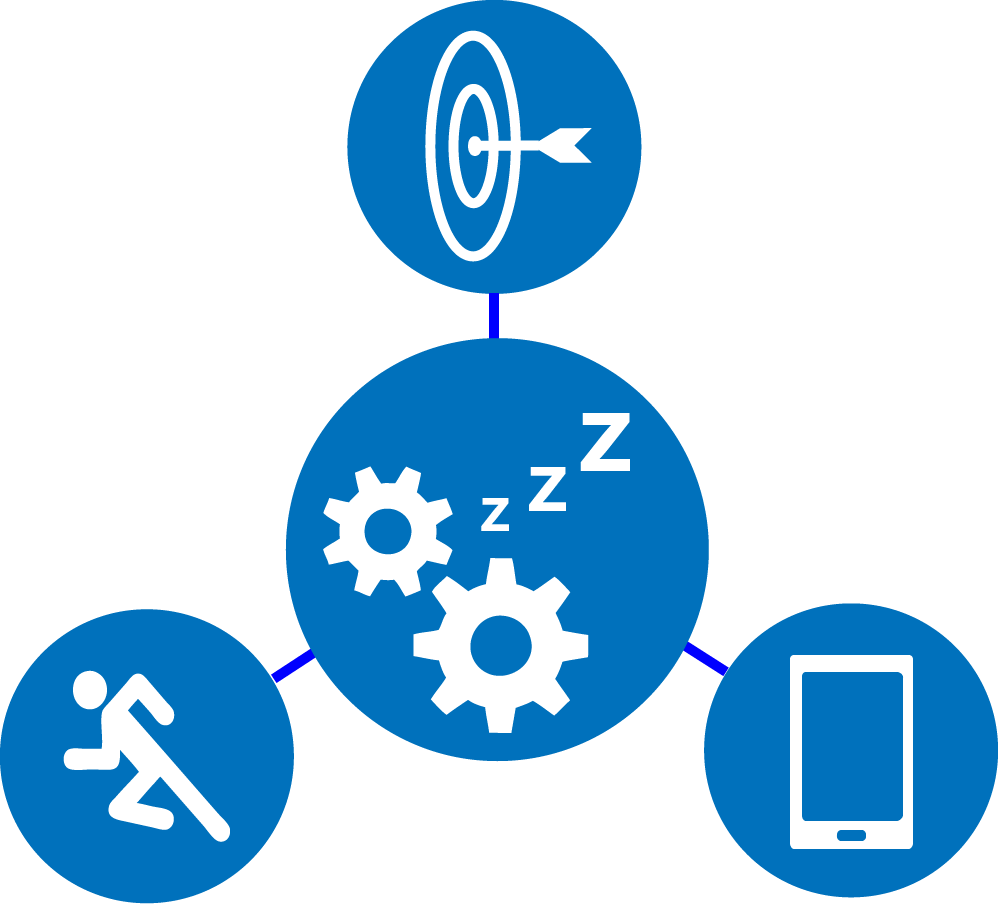
\includegraphics[width=4cm]{img/all}
    \caption[Schwerpuntke der Anwendung]{Die Anwendung mit den Schwerpunkten: Korrektheit, Portabilität und Komfort \label{fig:emphasis}}
  \end{center}
\end{figure}